\documentclass[a4j,12pt]{jarticle}
\usepackage[dvipdfmx]{graphicx}
\usepackage{amssymb}
\usepackage{amsmath}
\usepackage{float}
\usepackage{url}
\begin{document}
\begin{center}
\thispagestyle{empty}
\vspace*{5zh}
\huge
令和2年度 卒業論文\\[50pt]
{\Huge 論理的文章のアウトラインの作成を

支援するツールの開発}\\
[80pt]
\huge
指導教員 須田 宇宙 准教授\\[30pt]
千葉工業大学 情報ネットワーク学科\\[10pt]
須田研究室\\[60pt]
1632144 \hspace{70pt} 三浦 恋\\[75pt]
\end{center}
\vspace*{-2cm}
\begin{flushright} 
\huge
提出日 2020年1月--日
\end{flushright}

\newpage
\pagenumbering{roman}
\tableofcontents%目次
\newpage
\pagenumbering{arabic}
\section{緒言}
%目次を作る際は\verb+\tableofcontents+ と打ちます。\\
%新しいページに区切るときは\verb+\newpage+ と打ちます

%背景
大学で論文やレポートを書かなければならない大学生に対して,論理的な思考力や論理的文章作成能力の要求が高まっている.しかし,論文やレポートを書く際にアウトラインなどの事前準備をせずに文章の作成を行ってしまう学生が多く,論理的な文章にならないことが問題点として挙げられる.
そのため,レポートの書き方の指導や修正を行うライティングセンターの設置などが進められているが継続的な利用が必要とされている.また,論文や小説などの長文作成を支援するものとして,アウトラインプロセッサなどが存在する.

%問題点
しかし,一般に論文や小説などの長文を作成するためのツールとして,アウトラインプロセッサが使用されることが多い.
これは,文章を階層的に管理することに主眼が置かれており,学生にとって主張や根拠などが明確な一貫した文章を書く力を養うためのツールではないことが問題点となっている.

%目的
そこで本研究では,主張や根拠などが明確な一貫した論文やレポートを書くため,準備段階であるアカデミックアウトラインツールを開発することを目的としている.
\newpage
\section{アカデミックライティングについて}
\subsection{論文とは}
論文とはエッセイや小説のように自由な文章表現ではなく,一定の形式に備えた文章表現である.またテーマをもとに問題をたて,問題に対し様々な手法で分析,考察し,問題解決につながる新たな知見や検証を行い,その結果を報告するものが論文である\cite{ren1}.

\subsection{論文の書き方}
論文を書く流れとして主に4つ作業工程を繰り返し行うことで,より良い論文を書くことができる.また,4つの工程を以下に示す.
\begin{itemize}
  \item テーマを決める
  \item 下調べを行う
  \item アウトラインの作成する
  \item 執筆する
\end{itemize}
\subsubsection{テーマを決める}
どのようなテーマの論文を書くのかを決めるため,素朴な疑問や資料を読んだ際の疑問を大切にし,論文のテーマを決めていく.またテーマが既に決まっている場合はキーワードをもとに,図や表などを使って思考を整理し,論点を見いだし下調べに入る.

\subsubsection{下調べを行う}
論文のテーマが決まった場合テーマに関しての知識を得るため,似たテーマの論文を調べ知見を広げる必要がある.検索エンジンや本などで下調べを行う.文献等を調べる際は図書館での検索やデータベースによる検索をし,資料を収集する.また収集した資料を読み込み,疑問点などが出てきた際には2.2.1に戻りテーマについて思考の整理などを行う.論点が定まり,十分な情報が集まるまでテーマ決めと下調べを繰り返し行う.

\subsubsection{アウトラインの作成する}
下調べが終わり論文のテーマを決めることができた場合次に,作成する文章の骨組みである,アウトラインの作成を行う.紙に書き出すことやアウトラインプロセッサなどのソフトウェアを使用して,章や節で書く内容を箇条書きに近いかたちで書いていき,全体の文章構造を決めていく.またアウトラインの作成例を図\ref{fig:a}に示す.

\subsubsection{執筆する}
フォーマットやアウトラインをもとに,執筆を行う.アウトラインや整理した資料,行った実験や検証の結果をもとにアウトラインを更に細かく作成していき,アウトラインから文章を作成をしていく.そこで必要な情報があった際には調べ,アウトラインを修正し,文章作成を行う.また,文章の書き出しから完成まで,途中何度も書いた文章を添削,修正を行う必要がある.

\begin{figure}[h]
\begin{center}
 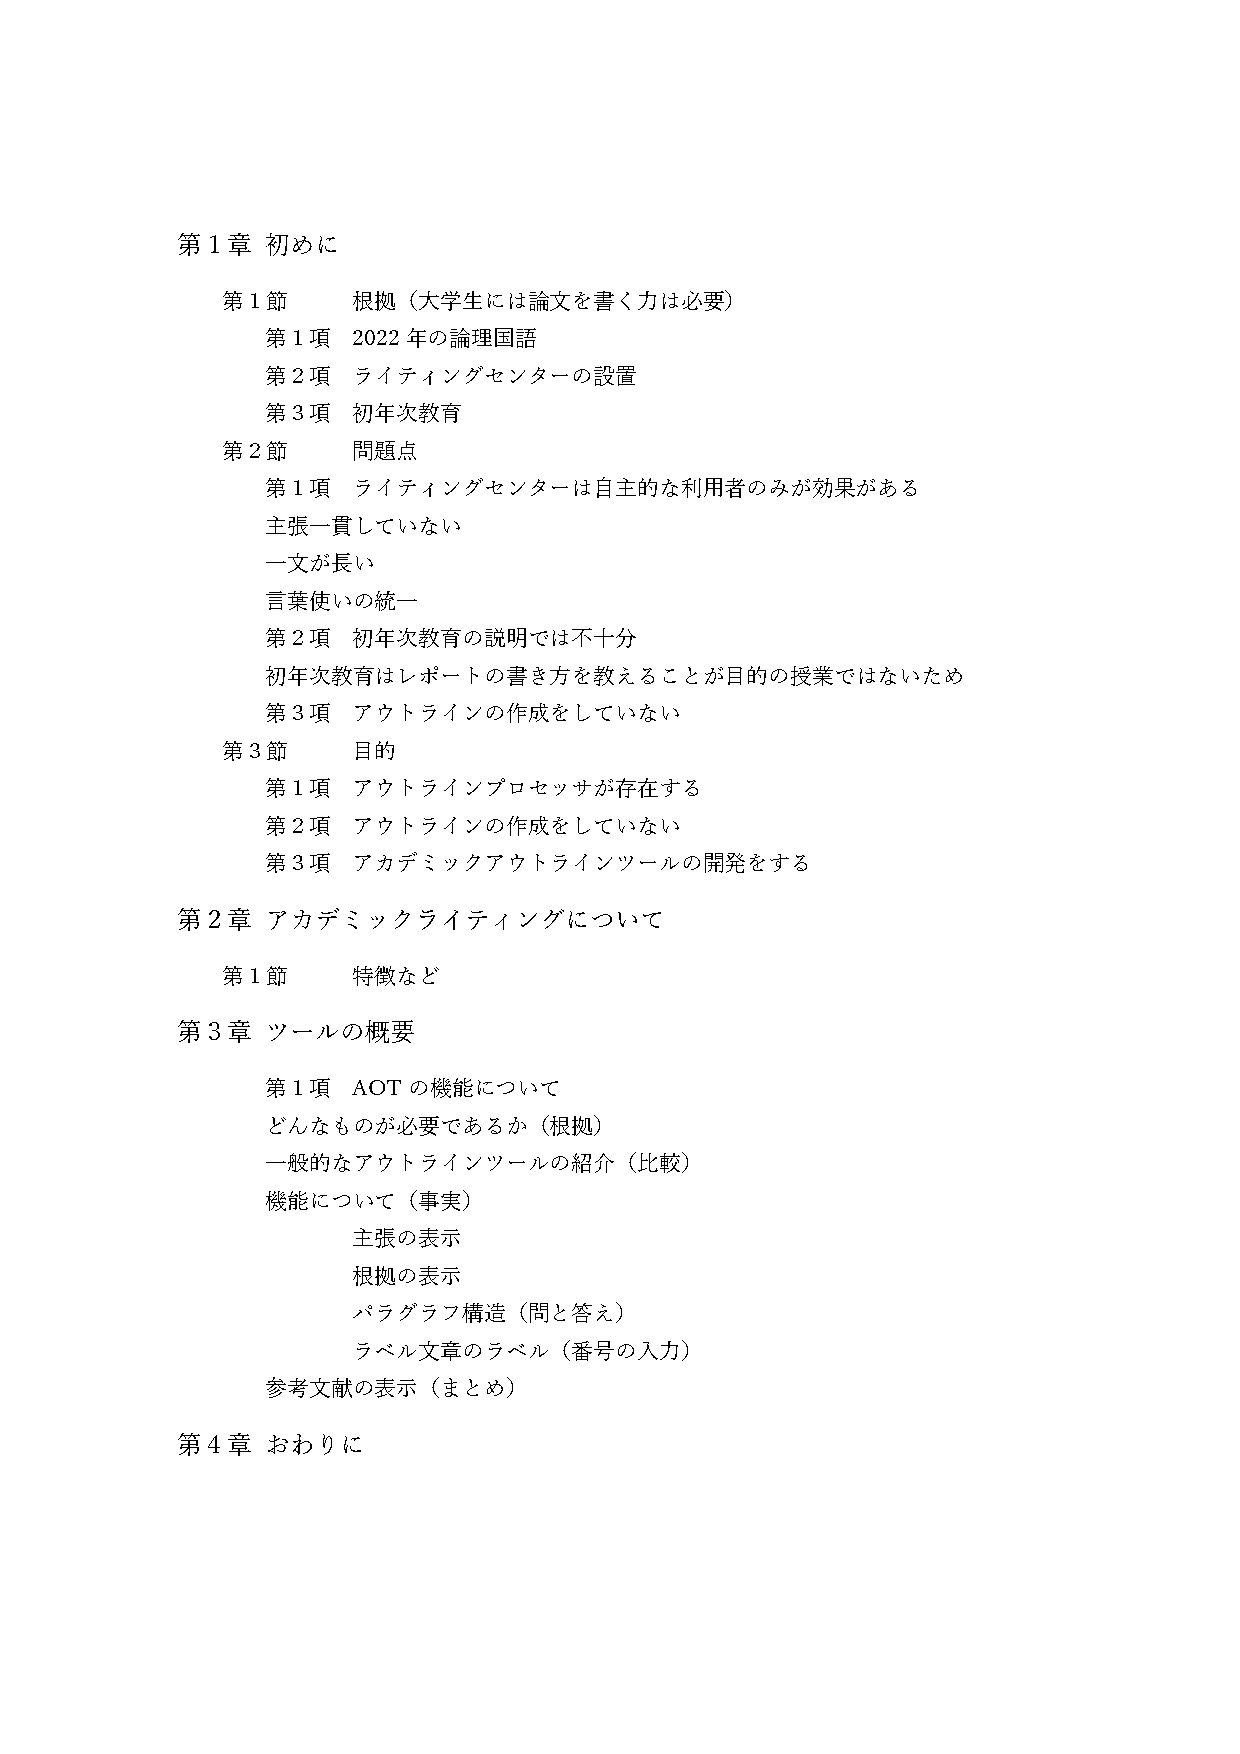
\includegraphics[scale=0.3]{outline.pdf}
\end{center}
 \caption{アウトラインの作成例}
 \label{fig:a}
\end{figure}
\newpage

\subsection{アカデミックライティングとは}
大学では答えのない問題を扱い,問題に対して自分の考えを主張することが必要とされている.そこで,大学で作成が求められる論文やレポート等には下記(1)〜(5)が求められる.このような文章を書く技術,書く行為はアカデミックライティングと呼ばれている\cite{ren2}.
\subsection{アカデミックライティングの特徴}
アカデミックライティングには重要な特徴として,以下の(1)〜(5)が挙げられる.
\begin{description}
  \item[(1)] 主張と根拠が明示されている
  \item[(2)] 問いと答えの構造と論理的な説明での構成されている
  \item[(3)] 引用の倫理のルールに従っている
  \item[(4)] パラグラフ構造になっている
  \item[(5)] 学術的文章に特有の一定の形式に従ってる
 \end{description}
 またアカデミックライティングは,専門的な内容を論じたり,まだ答えが発見されていないことについて論じることがあるため,複雑な概念や専門用語を用いて文章の作成を行う.しかし内容が読者に伝わらなければ文章の意味がなく,そのためにアカデミックライティングはわかりやすい文章で書く必要があることも特徴として挙げられる\cite{ren7}.
 
\subsection{なぜアカデミックライティングが必要がなのか}
大学では答えのない問題を扱うことが多く,授業ではレポート課題が出される.新たな発見をめざす研究やすでに分かっているが解釈が分かれたり,位置付けのはっきりしない事柄が多い.そのため答えのない問題について,学生がどの程度授業の内容を理解し,また自分なりの問いや答えを見つけることに努力を行ったかを確認するために課している.

\subsection{作文・感想文との違い}
同じ文章でもアカデミックライティングは作文や感想文とは大きく異なる.作成や感想文は自分の経験や思いを書くものであり,言葉遣いも話し言葉のような文体でも許される.しかし,アカデミックライティングは文献や調査結果などの根拠をもとに学術的なルールに従った報告書である.そのため,内容としては論理的な一貫した説明でなければならい.

\newpage
\section{論文などの作成を支援するソフトウェアや手法の紹介}
\subsection{アウトラインプロセッサ}
アウトラインプロセッサとは,一般的には小説などの長文を書く際に利用されている.
特徴として,見出しをつけ階層的に管理や位置の入れ替えなど行い,全体の構成を確認しながら文章の作成を支援するソフトウェアである.
%図の挿入をする予定
\subsection{TEX}
TeXとは,アメリカの著名な数学者にして計算機科学者であるDonald E. Knuthが作成した組版フリーソフトウェアである.TeX本体は,文字を配置する,基本的な組版作業に対応する命令を処理するものであり,命令だけを用いて文書を作成するのは効率的ではない.そこで多くの場合マクロセットと呼ばれる命令セットを用いて文書を作成している.

マクロとは,組版された文書の作成を容易にするために,複数の基本的な命令を組み合わせて作成された新たな命令である.
マクロセットにはさまざまなものがあるが,もっとも有名でよく用いられているものが,アメリカの計算機科学者であるLeslieLamportが作成したLaTeXである.TeXで文書を作成するという場合,実際はこのLaTeXの命令を用いて作成することがほとんどである.

また,日本語で書かれた文章をTeXで組版するため,(株)アスキーにおいてASCII日本語TeXが,日本電信電話公社においてNTT JTeXがそれぞれ開発されたことにより,日本においてもTeXが普及し現在に至っている\cite{ren3}.
%図の挿入をする予定

\subsection{Microsoft Word}
WordとはMicrosoft社が提供する文章作成ソフトウェアである.Micosoft社がが販売するワープロソフトのことであり,ソフトウェアのパッケージ製品であるMicrosoft Officeの中でも,主要なソフトウェアの1つに挙げられる.また,文章作成だけでなく,図形描画やグラフ,アウトラインの作成など,豊富で様々な機能のを持つ.
%図の挿入をする予定?いる?
\newpage
\subsection{マインドマップ}
マインドマップとは,頭の中で自然に行っている思考のプロセスを反映したノート法である.イギリス人教育者であるトニー・ブザン (Tony Buzan)が1970年代に出演していたTV番組を始めとして様々な著作で「マインドマップ」という言葉が広め始めた\cite{ren4}.また,自由な思考,アイデアや情報の流れを中心となる概念から分岐させる形で描画した図である.描画することで,アイデアの整理,効果的なメモの作成,記憶の定着強化などを実現することが可能になる.%mainndomap zu 

\newpage
\section{実装技術}
\subsection{PWAとは}
PWA(Progressive Web Apps)とはモバイルサイト上でネイティブアプリのようなユーザー体験を提供する技術であり,ウェブとアプリの両方の良さを兼ね備えている.具体的にはインストールが必要なく,ホーム画面へのアイコン追加やプッシュ通知の可能であり,ユーザーとの接触機会を増やすことができる.また読み込み速度や表示の高速化,オフラインでの閲覧も可能であるなど様々なメリットが得られる.またアプリとの違いとして,アプリストアを経由してダウンロードやインストールする手間がなく,アプリの導入までの手順を短縮ができる.またプラットフォームごとに開発する必要も
なく1つのPWAを構築するだけで,デバイスを問わずに一貫した内容を表示できるなど開発の自由度が高い\cite{ren6}.
\newpage
\section{本研究で開発したツールの概要}
\subsection{実装理由}
%実装した機能がなぜひつようであるのか?コンセプトを書く
本制作では論理的文章を書く際の準備段階である,アウトラインの作成をにおいて主張と根拠の確認や参考文献の管理を行うことでアウトラインの作成や主張の一貫した文章の作成を支援することができるツールが必要であると考えた.また,通学時間などの隙間時間で意見や構成の整理を行うことでアウトラインの作成時間を短くし,論理的文章を書く時間の確保ができることを目指した.

\subsection{開発言語について}
開発言語として,自宅や学校のみならず隙間時間に利用することを視野に入れ,PC とスマートフォンの両
方からのアクセスによる利用を考えた.そこで Web 上で動作するツールが望ましいと考え,HTML5,CSS3, JavaScript を使用し開発を行った.
\subsection{実装した機能について}
本ツールで開発した機能は以下の4つの機能の開発を行った.
\begin{description}
  \item[1-1] 主張と根拠の明確化
  \item[1-2] 課題に対する疑問とその答えの記入
  \item[1-3] 論理的な構成の整理
  \item[1-4] 参考文献の管理
 \end{description}
%実際の画面を画像としてはる

\subsubsection{主張と根拠の明確化}
主張と根拠の明確化の機能は,アウトライン作成時に主張や根拠を表示させることで,アウトラインの作成や文章作成の際に確認を行い,主張からずれた意見が出ることを防ぐことができると考えこのような機能にした.
主張のテキストボックス内では課題に対した自分の主張を記入し,根拠のテキストボックスでは,下調べを行った際根拠となるものを記入する.

\subsubsection{課題に対する疑問とその答えの記入}
この機能では文章をアカデミックライティングの特徴である「問いと答え」の形式で記述を行うことで,文章に必要な情報などを明確化していくことができると考えこのような機能にした.また記入する内容としては,課題のテーマに対しての疑問とそれに対する自分の考えである答えをそれぞれ「問い」と「答え」の部分に記入してく.

\subsubsection{論理的な構成の整理}
この機能では,一般的なアウトラインプロセッサと同様に論理的な文章を書く上で各内容の順番や情報を整理するため順番を入れ替える機能,章や段落の情報を表示する機能にした.具体的にはボタンを押すことによって上下の内容が入れ替わる機能になっている.

\subsubsection{参考文献の管理}
文章を作成する際下調べなどで行った引用した文献や本などを確認, 整理する機能にした.

\newpage

\subsection{利用方法}
%図を使っての利用方法の説明を行う.
\subsubsection{画面構成}

\newpage

\section*{謝辞}

\addcontentsline{toc}{section}{謝辞}
ここに研究の謝辞.主にご協力いただいた方など.
\bibliographystyle{jplain}
\newpage
\addcontentsline{toc}{section}{参考文献}
 \begin{thebibliography}{99}
\bibitem{ren1}山崎 憲一,萬代 雅希"論文とは",電子情報通信学会 通信ソサイエティマガジン,2016年9巻4号216-221.
\url{https://www.jstage.jst.go.jp/article/bplus/9/4/9_216/_pdf}

\bibitem{ren2} 堀 一成,坂尻 彰宏:"阪大生のためのアカデミックライティング",
\url{https://ir.library.osaka-u.ac.jp/repo/ouka/all/27153/Academic%20Writing%20Introduction.pdf}, 2019/8/23参照
\bibitem{ren3} 山本 浩: "TeXを使った論文作成方法",2000年103巻984号770-773.
\url{https://www.jstage.jst.go.jp/article/jsmemag/103/984/103_KJ00001459868/_article/-char/ja/}
\bibitem{ren4} "Lucidchart,5分でわかる、マインドマップの書き方と意味"
\url{https://www.lucidchart.com/pages/ja/mind-map#section_0}
\bibitem{ren5} "マインドマップの学校"
\url{https://www.mindmap-school.jp/mindmap/mindmap-law/}
\bibitem{ren6} "ディーエムソリューションズ株式会社"
\url{https://digital-marketing.jp/seo/what-is-progressive-web-apps/#i-6}
\bibitem{ren7} "早稲田ウィークリー,特集"
\url{https://www.waseda.jp/inst/weekly/feature/2014/06/23/20860/}
\end{thebibliography}
\section*{付録}

\addcontentsline{toc}{section}{付録}

\end{document}
